\documentclass[14pt]{thapathali}
\usepackage{colortbl}
\usetikzlibrary{positioning}

% ============================================
% CUSTOMIZABLE VARIABLES - Edit these
% ============================================
\projecttitle{Multi-Agent Data Analysis and Insight Generation Platform For Financial and Sales Data}
\projectsubtitle{Mid-Progress Presentation}

\newcommand{\studentone}{Prashant Kafle}
\newcommand{\rollone}{THA080BCT026}
\newcommand{\studenttwo}{Roshan Poudel}
\newcommand{\rolltwo}{THA080BCT036}
\newcommand{\studentthree}{Santosh Khadka}
\newcommand{\rollthree}{THA080BCT039}
\newcommand{\studentfour}{Sushil Bhatta}
\newcommand{\rollfour}{THA080BCT048}

\presentername{\studentone}
\studentroll{\rollone}
\supervisorname{Er. Rajad Shakya}
\supervisortitle{Lecturer}
\departmentname{Department of Electronics and Computer Engineering}
\institutionname{Institute of Engineering, Thapathali Campus}
\presentationdate{17 July, 2026}
\academicyear{Academic Year: 2024/2025}

% ============================================
% TITLE PAGE SETUP
% ============================================
\csname title\endcsname[\ProjectTitle]{\ProjectTitle}
\subtitle{\ProjectSubtitle}
\author[\studentone]{\studentone, \studenttwo, \studentthree, \studentfour}
\institute[\DepartmentName]{\DepartmentName}
\date[\PresentationDate]{\PresentationDate}

% ============================================
% DOCUMENT BEGINS
% ============================================
\begin{document}

% ============================================
% TITLE SLIDE
% ============================================

\begin{frame}[plain]
    \vspace{0.8cm}

    % Title - large, bold, centered, uppercase
    \begin{center}
        {\Large \bfseries \MakeUppercase{\ProjectTitle} \par}
    \end{center}

    \vspace{1em}

    % Team Members (left) and Supervisor (right)
    \begin{columns}[t, onlytextwidth]
        \begin{column}{0.55\textwidth}
            \hspace{1em}{\normalsize \bfseries Team Members:}\par
            \vspace{0.3em}
            \hspace{1em}{\small \studentone{} (\rollone)}\\[2pt]
            \hspace{1em}{\small \studenttwo{} (\rolltwo)}\\[2pt]
            \hspace{1em}{\small \studentthree{} (\rollthree)}\\[2pt]
            \hspace{1em}{\small \studentfour{} (\rollfour)}
        \end{column}

        \begin{column}{0.4\textwidth}
            \raggedleft
            {\normalsize \bfseries Supervised By:}\par
            \vspace{0.3em}
            {\small \SupervisorName}\par
        \end{column}
    \end{columns}

    \vfill

    % Department and institution centered at bottom
    \begin{center}
        {\normalsize \DepartmentName}\par
        {\normalsize \InstitutionName}\par
        \vspace{0.3em}
        {\normalsize \PresentationDate}
    \end{center}

    \vspace{0.5cm}
\end{frame}

% ============================================
% PRESENTATION OUTLINE
% ============================================
\begin{frame}{Presentation Outline}
    \begin{columns}[t, onlytextwidth]
        \begin{column}{0.48\textwidth}
            \begin{itemize}
                \item Introduction
                \item Methodology
                \item Current Progress
            \end{itemize}
        \end{column}
        \begin{column}{0.48\textwidth}
            \begin{itemize}
                \item Verified Outputs
                \item Current Limitations
                \item Remaining Work and Timeline
                \item Conclusion
                \item References
            \end{itemize}
        \end{column}
    \end{columns}
\end{frame}

% ============================================
% MOTIVATION
% ============================================

\begin{frame}{Motivation}
    \begin{itemize}
        \item Despite the availability of data, many organizations lack the technical expertise required to analyze and interpret it effectively.
        \item Traditional data analysis tools often require statistical knowledge, programming skills, or manual report interpretation.
        \item Existing AI-based systems using LLMs may generate unverified or hallucinated insights, leading to unreliable conclusions.
    \end{itemize}
\end{frame}

% ============================================
% INTRODUCTION
% ============================================

\begin{frame}{Introduction}
    \begin{itemize}
        \item The project is being implemented as a state-based data analysis pipeline for sales and financial CSV datasets.
        \item Four pipeline stages are currently connected: structural profiling, semantic tagging, preprocessing, and statistical analysis.
        \item The system transforms raw records into a cleaned dataset, a preprocessing audit trail, quality metrics, statistics, and chart files.
        \item Mathematical operations are performed with Python libraries; the language model is used for semantic interpretation and processing rules.
        \item The current implementation provides a working backend foundation for the planned user-facing platform.
    \end{itemize}
\end{frame}

% ============================================
% OBJECTIVES
% ============================================

\begin{frame}{Objectives}
    \begin{itemize}
        \item Develop an autonomous multi-agent system that converts raw sales and financial data into reproducible analytical outputs.
        \item Implement semantic, context-aware preprocessing instead of applying the same cleaning rule to every column.
        \item Evaluate the pipeline using representative datasets, focused unit tests, and generated diagnostics.
        \item Establish a reliable backend foundation before completing report generation and the user interface.
    \end{itemize}
\end{frame}

% ============================================
% SCOPE OF PROJECT
% ============================================

\begin{frame}{Scope of Project}
    \begin{itemize}
        \item Focus on financial and sales datasets (CSV/Excel format)
        \item Automated data cleaning, preprocessing, and validation
        \item Financial statistical analysis (profit, revenue, trends)
        \item Multi-agent system for structured financial analysis workflow
        \item Insight generation with natural language explanations
        \item Validation of financial insights to reduce hallucination and Report Generation
    \end{itemize}
\end{frame}

% ============================================
% METHODOLOGY
% ============================================

\begin{frame}{Methodology -- Current 4-Stage Pipeline}
    \begin{center}
        
\includegraphics[width=\textwidth,height=0.74\textheight,keepaspectratio]{src/images/fiximag.png}
    \end{center}
\end{frame}

% ============================================
% AGENT 1
% ============================================
\begin{frame}{Agent 1 -- Raw Structural Profiler}
    \begin{columns}[T]
        \begin{column}{0.55\textwidth}
            \begin{itemize}
                \item Reads the input CSV and records shape, dtypes, missingness, uniqueness, and duplicates.
                \item Produces a raw structural profile without changing the source data.
                \item Caches the DataFrame for the downstream stages.
            \end{itemize}
        \end{column}
        \begin{column}{0.42\textwidth}
            \centering
            
\includegraphics[width=\linewidth,height=0.80\textheight,keepaspectratio]{src/images/agent1pic.png}
        \end{column}
    \end{columns}
\end{frame}

% ============================================
% AGENT 2
% ============================================
\begin{frame}{Agent 2 -- Technical Inference \& Semantic Tagging}
    \begin{columns}[T]
        \begin{column}{0.55\textwidth}
            \begin{itemize}
                \item Sniffs numeric, datetime, boolean, and string types using local heuristics.
                \item Uses Groq-based semantic tagging when available and falls back to deterministic rules when it is not.
                \item Creates a per-column blueprint containing type, semantic tag, scaling, imputation, and analysis policies.
                \item Passes the blueprint to preprocessing instead of hard-coding one rule for every column.
            \end{itemize}
        \end{column}
        \begin{column}{0.42\textwidth}
            \centering
            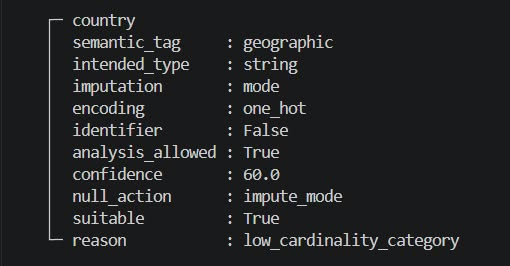
\includegraphics[width=\linewidth,keepaspectratio]{src/images/agent2pic.png}
        \end{column}
    \end{columns}
\end{frame}

% ============================================
% AGENT 3
% ============================================
\begin{frame}{Agent 3 -- Context-Aware Preprocessing}
    \begin{columns}[T]
        \begin{column}{0.55\textwidth}
            \begin{itemize}
                \item Coerces columns according to the semantic blueprint and cleans international currency formats.
                \item Standardizes text and null variants while preserving identifiers.
                \item Removes duplicates, applies configured imputation, and clips permitted outliers with IQR bounds.
                \item Extracts date features and derives metrics such as profit, margin, and revenue per unit.
                \item Records scaling parameters, an audit log, and a 0--100 data quality score.
            \end{itemize}
        \end{column}
        \begin{column}{0.42\textwidth}
            \centering
            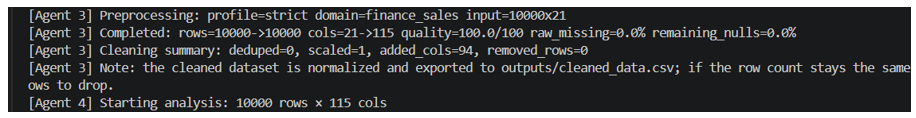
\includegraphics[width=\linewidth,height=0.80\textheight,keepaspectratio]{src/images/agent3pic.png}
        \end{column}
    \end{columns}
\end{frame}

% ============================================
% AGENT 4
% ============================================
\begin{frame}{Agent 4 -- Visualization \& Statistical Analysis}
    \begin{columns}[T]
        \begin{column}{0.55\textwidth}
            \begin{itemize}
                \item Calculates descriptive statistics, correlations, distributions, growth, and seasonality.
                \item Detects anomalies using a configurable z-score threshold.
                \item Computes regression trends and category rankings when the dataset supports them.
                \item Saves reproducible PNG charts and structured statistics to the pipeline state.
            \end{itemize}
        \end{column}
        \begin{column}{0.42\textwidth}
            \centering
            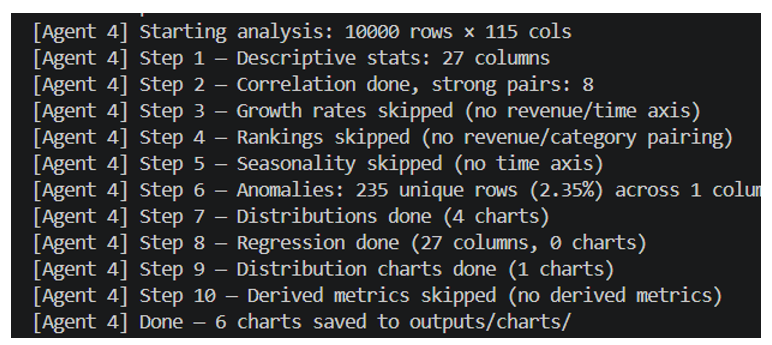
\includegraphics[width=\linewidth,keepaspectratio]{src/images/agent4pic.png}
        \end{column}
    \end{columns}
\end{frame}

% ============================================
% AGENT 5
% ============================================

% ============================================
% RESULT
% ============================================

\begin{frame}{Current Progress -- Verified Run}
    \begin{itemize}
        \item \textbf{Input tested:} Amazon sales CSV with 10,000 rows and 21 columns.
        \item \textbf{Agent 1:} 210,000 cells profiled; 0 missing cells and 0 duplicate rows in the run.
        \item \textbf{Agent 2:} All 21 columns received a semantic schema blueprint and processing policy.
        \item \textbf{Agent 3:} Cleaned CSV, scaling parameters, column ledger, preprocessing log, and quality metrics generated.
        \item \textbf{Agent 4:} Statistics and chart infrastructure executed through the LangGraph pipeline.
    \end{itemize}
\end{frame}

\begin{frame}{Generated Outputs}
    \begin{itemize}
        \item Cleaned dataset exported to \texttt{backend/outputs/cleaned\_data.csv}
        \item Run metadata exported to \texttt{agent\_run\_diagnostics.json}
        \item Correlation heatmap and numeric distribution charts generated as PNG files
        \item Category and payment-method distribution charts generated from the processed data
        \item Reliability metadata records stage confidence, evidence, and decision readiness
    \end{itemize}
\end{frame}


% ============================================
% ANALYSIS
% ============================================

\begin{frame}{Current Analysis}
    \begin{itemize}
        \item \textbf{Deterministic analysis:} Pandas, NumPy, SciPy, and Matplotlib perform the numeric calculations and visualizations.
        \item \textbf{Semantic flexibility:} The schema blueprint lets preprocessing respond to column meaning while retaining a fallback path when the LLM is unavailable.
        \item \textbf{Traceability:} The pipeline preserves an audit log, scaling parameters, quality metrics, charts, and diagnostics for each run.
        \item \textbf{Current boundary:} The backend is functional, but the final validation agent, natural-language report assembly, and user interface are not complete yet.
    \end{itemize}
\end{frame}

% ============================================
% SECTION 14: PROJECT TIMELINE
% ============================================

\begin{frame}{Mid-Progress Timeline}
    \begin{itemize}
        \item \textbf{Completed:} project architecture, GraphState, Agents 1--3, conditional pipeline routing, preprocessing audit trail, quality scoring, and focused tests.
        \item \textbf{Current:} Agent 4 statistical analysis and chart generation, verified on the Amazon sales dataset.
        \item \textbf{Next:} connect statistics to evidence-backed insight generation.
        \item \textbf{Final phase:} upload workflow, frontend presentation, broader datasets, and end-to-end evaluation.
    \end{itemize}
\end{frame}

\begin{frame}{Remaining Work}
    \begin{center}
        \begin{tabular}{p{0.32\textwidth} p{0.52\textwidth}}
            \textbf{Work package} & \textbf{Target outcome} \\
            \hline
            Validation guardrail & Cross-check statistics, charts, and evidence \\
            Insight generation & Produce traceable natural-language findings \\
            Interface & Upload data and display progress/results \\
            Evaluation & Benchmark accuracy, robustness, and runtime
        \end{tabular}
    \end{center}
\end{frame}

% ============================================
% CONCLUSION
% ============================================

\begin{frame}{Conclusion}
    \begin{itemize}
        \item \textbf{Fixing Waste Data:} The system successfully proves that raw, ignored spreadsheets can be turned into valuable, easy-to-read reports automatically.
        \item \textbf{Beating Local Challenges:} By using free, open-source technology, it solves major real-world problems like high software costs and a lack of local tech experts in rural areas.
        \item \textbf{Reliable Design:} It blends rock-solid mathematical rules with creative AI explanations inside a safe, structured pipeline.
    \end{itemize}
\end{frame}

% ============================================
% REFERENCES
% ============================================

\begin{frame}[allowframebreaks]{References}
    \begin{enumerate}
        \scriptsize
        \item Y.~K. Dwivedi, L. Hughes, A.~M. Baabdullah, et al., ``So what if ChatGPT wrote it? Multidisciplinary perspectives on opportunities, challenges and implications of generative conversational AI for research, practice and policy,'' \textit{International Journal of Information Management}, vol. 71, 2023.
        \item OpenAI, ``GPT-4 Technical Report,'' 2024.
        \item M. Sun, R. Han, B. Jiang, H. Qi, D. Sun, Y. Yuan, and J. Huang, ``LAMBDA: A Large Model Based Data Agent,'' \textit{arXiv preprint arXiv:2407.17535}, 2024.
        \item Y.~K. Liu, et al., ``Summary of ChatGPT-Related Research and Perspective Towards the Future of Large Language Models,'' \textit{arXiv:2306.07209}, 2023.
        \item J. Maynez, S. Narayan, B. Bohnet, and R. McDonald, ``On Faithfulness and Factuality in Abstractive Summarization,'' in \textit{Proceedings of ACL}, 2020.
        \item V. Dibia and C. Demiralp, ``Data2Vis: Automatic Generation of Data Visualizations Using Sequence-to-Sequence Recurrent Neural Networks,'' \textit{IEEE Computer Graphics and Applications}, vol. 39, no. 5, pp. 33--46, 2019.
        \item K. Hu, M.~A. Bakker, S. Li, T. Kraska, and C.~A. Hidalgo, ``VizML: A Machine Learning Approach to Visualization Recommendation,'' in \textit{Proceedings of the CHI Conference}, 2019.
        \item D. Moritz, C. Wang, G.~L. Nelson, H. Lin, A.~M. Smith, B. Howe, and J. Heer, ``Formalizing Visualization Design Knowledge as Constraints,'' \textit{IEEE Transactions on Visualization and Computer Graphics}, 2018.
        \item Y. Luo, X. Qin, N. Tang, and G. Li, ``DeepEye: Towards Automatic Data Visualization,'' in \textit{IEEE ICDE}, 2018.
        \item LangChain, ``LangGraph: A Python Library for Building Stateful, Multi-Agent Applications,'' 2024.
        \item Q. Wu, G. Bansal, J. Zhang, et al., ``AutoGen: Enabling Next-Gen LLM Applications via Multi-Agent Conversation Framework,'' 2023.
        \item Z. Ji, et al., ``Survey of Hallucination in Natural Language Generation,'' \textit{ACM Computing Surveys}, 2023.
        \item G. Li, et al., ``CAMEL: Communicative Agents for `Mind' Exploration of Large Language Model Society,'' \textit{arXiv:2303.17760}, 2023.
        \item N. Shinn, et al., ``Reflexion: Language Agents with Verbal Reinforcement Learning,'' \textit{arXiv:2303.11366}, 2023.
        \item D.~P. Kingma and J. Ba, ``Adam: A Method for Stochastic Optimization,'' \textit{ICLR}, 2015.
        \item E.~J. Hu et al., ``LoRA: Low-Rank Adaptation of Large Language Models,'' \textit{ICLR}, 2022.
    \end{enumerate}
\end{frame}


\end{document}
